% LaTeX template for Lab Reports
% Copyright (C) 2014 Julian Coy

%% CHANGE REPORT TITLE HERE
\newcommand{\reporttitle}{
 FSM System Design
}

%% HEADER/PREAMBLE INFORMATION

% "The font should be 11pt Times New Roman"
\documentclass[11pt]{report}
\usepackage[T1]{fontenc}
\usepackage[utf8]{inputenc}

\usepackage{mathptmx}               

% "The body of the paper should use 1" margins on all sides."
\usepackage[margin=1in]{geometry}

% "Pages must be numbered, starting with 1 on the first page in the body of the report.
% The cover page should not be numbered. 
% Page numbers should be in the bottom-right corner of the page."
\usepackage{fancyhdr}
\pagestyle{fancy}
\fancyhead{}
\fancyfoot{}
\renewcommand{\headrulewidth}{0pt}
\fancyfoot[R]{\thepage}

% Set up customized spacing
\usepackage{setspace}

% Allows for Trademark Symbols
\usepackage{textcomp}

% Remove spacing between items in lists
\usepackage{enumitem}

% Remove extra spacing between titles of sections and subsections
\usepackage{titlesec}
\titlespacing\section{0pt}{10pt}{10pt}
\titlespacing\subsection{0pt}{10pt}{10pt}
\titlespacing\subsubsection{0pt}{0pt plus 4pt minus 2pt}{0pt plus 2pt minus 2pt}

% Setup the specialized chapter section for the Abstract
\titlespacing\chapter{0pt}{0pt plus 4pt minus 2pt}{0pt plus 2pt minus 2pt}
\titleformat{\chapter}[block]{\centering\Huge}{}{}{}{}

% Set up BibTeX integration using IEEE citation format
\usepackage{cite}
\bibliographystyle{ieeetr}
\usepackage{url}

% Set bibliography to have a section header rather than chapter header
\makeatletter
\renewenvironment{thebibliography}[1]
     {\section*{\scshape Works Cited}% <-- this line was changed from \chapter* to \section*
      \@mkboth{\MakeUppercase\bibname}{\MakeUppercase\bibname}%
      \list{\@biblabel{\@arabic\c@enumiv}}%
           {\settowidth\labelwidth{\@biblabel{#1}}%
            \leftmargin\labelwidth
            \advance\leftmargin\labelsep
            \@openbib@code
            \usecounter{enumiv}%
            \let\p@enumiv\@empty
            \renewcommand\theenumiv{\@arabic\c@enumiv}}%
      \sloppy
      \clubpenalty4000
      \@clubpenalty \clubpenalty
      \widowpenalty4000%
      \sfcode`\.\@m}
     {\def\@noitemerr
       {\@latex@warning{Empty `thebibliography' environment}}%
      \endlist}
\makeatother

% Set up math
\usepackage{amsmath}
\usepackage{amsfonts}
\usepackage{amssymb}

% Set up graphics
\usepackage{graphicx}
\usepackage{float}

% Set up tables
\usepackage{tabularx}
\usepackage{booktabs}

% Set up code blocks
% or not...

\usepackage{listings}
\usepackage{color}

\definecolor{dkgreen}{rgb}{0,0.6,0}
\definecolor{gray}{rgb}{0.5,0.5,0.5}
\definecolor{mauve}{rgb}{0.58,0,0.82}

\lstset{frame=tb,
  language=VHDL,
  aboveskip=3mm,
  belowskip=3mm,
  showstringspaces=false,
  columns=flexible,
  basicstyle={\small\ttfamily},
  numbers=none,
  numberstyle=\tiny\color{gray},
  keywordstyle=\color{blue},
  commentstyle=\color{dkgreen},
  stringstyle=\color{mauve},
  breaklines=true,
  breakatwhitespace=true
  tabsize=3
}

%% START OF DOCUMENT

\begin{document}

% "The main body of text should use 1.5 spacing"
\begin{spacing}{1.5}

% Suppress page numbering on first page
\thispagestyle{empty}

\begin{scshape}

% Title
% "The title should be centered and written in approximately 22pt font."
\vspace*{30pt}
{
\Huge
\begin{center}
    \reporttitle
\end{center}
}
\vspace{30pt}

% Team Number
% "The Team number should be centered and written several lines below the title and should use a
% similar size font as the title."
{
\Large
\begin{center}
  Lab Report 2 for ECE327 \\
  Digital Systems Design
\end{center}
}
\vspace{30pt}
% Team Members
% "Directly below the team identifier, team members should be listed alphabetically by last name, one
% per line, in approximately 14pt font. The column of names should be approximately centered on
% the page, but the names within the column should be left justified (so they all start at the same
% horizontal position)."
{
\Large 
\begin{center}
  Submitted by \\
  Julian Coy
\end{center}
}
\vspace{120pt}

{
\Large
\begin{center}
  Undergraduate of Electrical \& Computer Engineering \\
  Clemson University
\end{center}
}
\vspace{30pt}

{
\Large
\begin{center}
  March 12, 2014
\end{center}
}

\end{scshape}

% New page and reset page numbering
\clearpage
\setcounter{page}{1}

%% START EDITS BELOW %%

\vspace{15pt}
  \setcounter{chapter}{1}
  \chapter*{Abstract}
  \label{cha:abstract}
\vspace{72pt}

Finite state machines (FSMs) are the basic building blocks of complex computing.  They allow for logical implementation of algorithms, which is critical to the engineering of computing systems.  In this lab, a finite state machine is constructed to flag "stop codons" in a sample of DNA code.  The implementation of this finite machine is done though VHDL using behavioral modeling techniques.  Testbench results are provided later in this report to show a working simulation of the FSM when connected to other logical components.  The other logical components built for this lab are a Parallel-to-Serial Output (PISO) register and a counter register.  The inputs to the FSM design will be threefold.  There will be one array of 18 switches which are used to simulate the DNA input.  There will also be a "reset" button and a "load" button.  The reset button will asynchronously reset the counter block, while the load button will be used to push new data into the PISO register. This design showcases the power of finite state machine logic.  It is critical for engineers to grasp the power of logical computation and to see the scalability of such power.  By combining simple FSM logical blocks, one can create a vast and complicated algorithm with ease.

\clearpage

\section*{\scshape Introduction} %(0.5 pages)
\label{cha:introduction}

The purpose of this lab is to sequence DNA bases consisting of T, A, C, and G and look for stop codons.  Stop codons are series of three bases that trigger the end of a DNA sequence.  The stop codons we look for in this lab are TAA, TGA, and TAG.  In order to differentiate the bases, we use a binary representation for the bases (Figure \ref{fig:bases}).  The bases are then fed into the FSM, the number of stop codons are counted, and then the count is displayed on the Altera board.

\vspace{15px}
\begin{figure}[H]
    \centering
    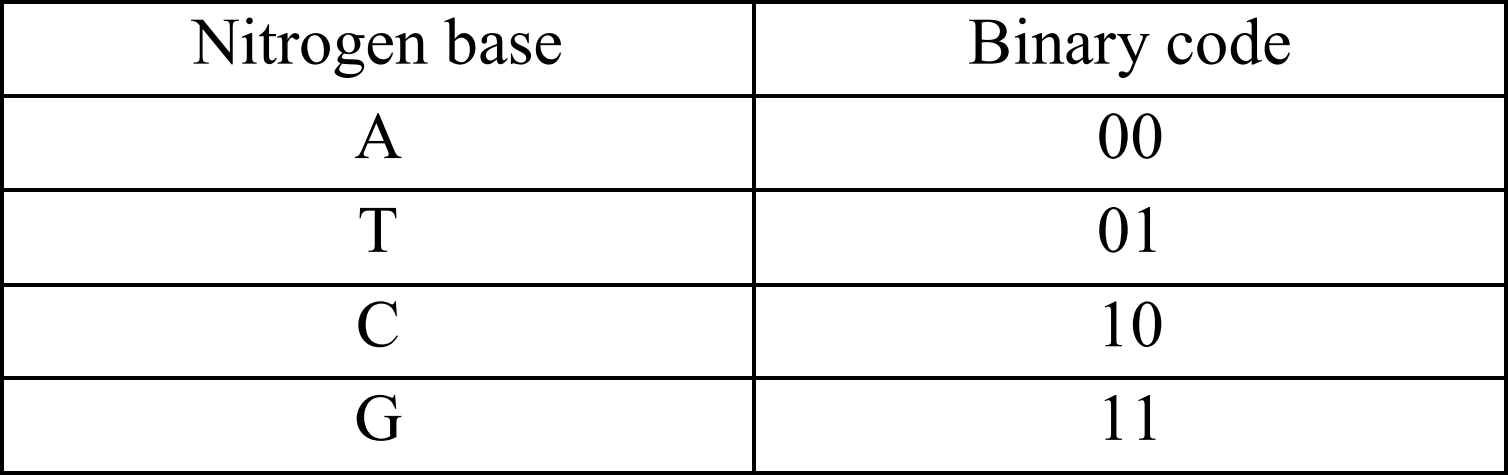
\includegraphics[width=0.6\textwidth,keepaspectratio]{bases}
    \caption{DNA Base Representation}
    \label{fig:bases}
\end{figure}

Lab two consists of three major logical components (the FSM logic, the counter logic, and the PISO logic) and one mior component (the LED logic).  The counter and PISO components are standalone and can be simulated through ModelSim for testing or used for implementation with other systems with minimal modifications.  The FSM logic is designed to model state transitions of the incoming DNA data from the PISO.  And the minor LED logic simply displays a number of LEDs correspondent to the output of the counter logic.

\section{\scshape FSM System Design} %(0.5 pages)
\label{sec:fsm_design}

\subsection{\scshape PISO Logic Design}
\label{sub:design_piso}

The PISO design for this lab was built specifically to handle 18 bits of input data at a time.  This was a design choice made for the layout of the Altera board, as it only allowed for 18 bits of modifiable input at a time. The PISO logic parses the 18 bits of data by 2 bit intervals.  It then outputs the first two bits of data on the rising edge of the clock.  This output is connected to the FSM input.  The PISO then shifts the data left by two bits and adds a "01" to the right end.  The "01" code was chosen for the shift packing to make sure that when the data is fully read, no extra stop codons are accidentally detected.  Since the code for the T base is "01" and no stop codons end with T or consist of all T's, this eliminates that possibility.

\subsection{\scshape Testing of the PISO}
\label{sub:test_piso}

To test the PISO, a teshbench was created that would send in different strings of data to the PISO and monitor the output on the rising edge of the following clock cycles.

\subsection{\scshape Counter Logic Design}
\label{sub:design_counter}

The counter is modeled behaviorally and simply counts the number of stop flags from the FSM it encounters.  The maximum count used for this project is three, but can be modified to much larger ranges with only a few lines of code.  The counter outputs its value on an integer signal that is sent to the LED logic.

\subsection{\scshape Testing of the Counter}
\label{sub:test_counter}

The counter was tested by sending stop flags to the input and periodically sending a reset signal.  The counter performed without issue even when using large integer values.  The maximum count size tested was 255, but since the maximum number of stop codones possible from the board were three, the counter integer limit was set to 3.

\vspace{30px}
\begin{figure}[H]
    \centering
    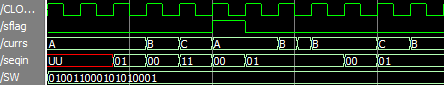
\includegraphics[width=1.0\textwidth,height=4cm]{simulation}
    \caption{Simulation Results\cite{Synth}}
    \label{fig:testbench}
\end{figure}


\subsection{\scshape Testing of the 2-to-1 Multiplexer}
\label{sec:test_2to1}

Testing of the multiplexer was done with a testbench through ModelSim.  Inside the test bench the input signals were initialized and set to different values.  Next, the channels were cycled through using the select signal.  Once cycled, the signal that was selected was changed and the change was verified through the Wave view in ModelSim.  Finally, the signal that was not selected was changed and monitored to make sure the output did not change.

Once the testbench was completed, the code was compiled inside of Quartus II and flashed onto the Cyclone IV FPGA.  Once the code was loaded onto the FPGA the switches and LEDS were used to verify the operation of the code.  For this multiplexer design, the switches 15 to 8 were used for the Y channel and switched 7 to 0 were used for X.  Switch 16 was used as the select signal and the red LEDs were connected to the output channel.  By toggling through the earlier mentioned states, the program was verified in hardware.

\section{\scshape 5-to-1 Multiplexer} % (fold)
\label{sec:5to1}

\subsection{\scshape Designing the 5-to-1 Multiplexer} % (fold)
\label{sub:design_5to1}

The second system was a 5-to-1 multiplexer design.  This design is very similar to the previous system.  The addition of three more channels will require a more complex decoding algorithm.  This can complicate the design greatly; however, smart implementation techniques can limit the overhead of the computation.  As shown in Figure a simple case block was sufficient to perform the select signal decoding for the 3 bit select line.  This method is inefficient with larger select lines as they exponentially increase the number of required cases per select channel bit.

\subsection{\scshape Testing the 5-to-1 Multiplexer} % (fold)
\label{sub:test_5to1}

The testing of the 5-to-1 multiplexer was almost exactly the same as the test for the 2-to-1.  Figure shows the timing diagram of the signals.  The diagram shows the transition from the output signal (TESTM) as the select signal (TESTS) is modified.  The first 5 changes for TESTS show the value of the output matching the selected input.  The second to last change shows that non-selected input does not affect the output.  The final change to TESTW when it is selected shows that the output changes immediately with the selected signal.


\section{\scshape Seven Segment Decoder}
\label{sec:seven_segment_decoder}

\subsection{\scshape Designing the Seven Segment Decoder} % (fold)
\label{sub:design_ssd}

% \vspace{30px}
% \begin{figure}[H]
%     \centering
%     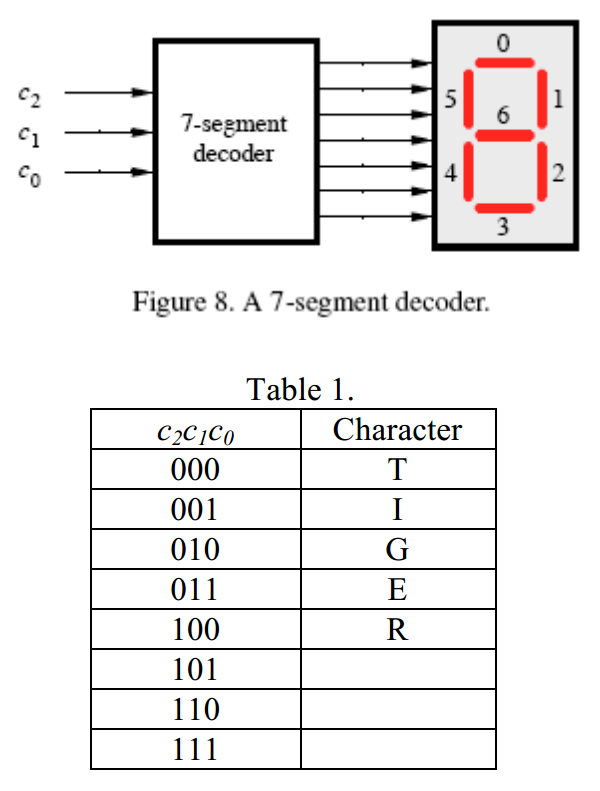
\includegraphics[width=0.3\textwidth]{ssd}
%     \caption{Seven Segment Display Logic}
%     \label{fig:ssd}
% \end{figure}

The basic truth table and signal layout for the seven segment decoder (SSD) are shown in Figure (ref here).  The SSD is supposed to take a 3-bit input and display a letter corresponding to the values in the truth table.  This means that a maximum of $2^3$  Each segment in the decoder is set by a bit.  So the input channel must be 7 bits wide to accommodate the SSD.

\subsection{\scshape Testing the Seven Segment Decoder} % (fold)
\label{sub:test_ssd}

Testing of the SSD is more efficient on the Cyclone IV due to the nature of the visual display.  For a human eye the waveform simulation was unfortunately hard to follow.  Although the waveform allowed for proper logical adjustments, it was unknown that the SSD required a low bit to activate a segment and all of the letters were inverted.  Figure shows the timing waveform.

\section{\scshape 5-Seven Segment Display}
\label{sec:5_ssd}

\subsection{\scshape Designing the 5-Seven Segment Display} % (fold)
\label{sub:design_5_ssd}

The final system of Lab 1 is a 5-count SSD that can display a word.  The word must be able to be shifted by a 3-bit select channel and each letter must be modifiable by another 3-bit select channel.  Each of the previous subsystems is included for the final design.  There are 5 5-to-1 multiplexers which are connected to SSDs.   

Figure shows the truth table for the select line input.  This table is assuming that the SSD letter codes are not changing when the select line does.  Each SSD also has a 3-bit select line that will tell the multiplexer what values to send to the decoder.  The diagram for the signals is shown in Figure .

\subsection{\scshape Testing the 5-Seven Segment Display}
\label{sub:test_5_ssd}

As the complexity of a system grows, so does the complexity of its verification.  The final system in lab 1 required multiple tests between components and tests of the components themselves to verify functionality.  For the test, the SSD were initialized to display "TIGER".  Then the letters were permuted through the TESTSW signal.  Once that was verified, the letters were randomized and then permuted randomly through the SSDs.  In the code the "default" value for the SSD was set to display the number "8" for easy debugging.

The code for the testbench can be seen in Appendix B.  The waveform simulation can be found in Appendix C.

\section{\scshape Conclusions} % (fold)
\label{sec:conclusions}

This lab is a testament to the modularity, reliability, and scope of FPGA programming with VHDL.  Simple components or systems can be designed and connected to form incredibly complex systems that can perform a wide range of actions.  Originally, the subsystems in the lab seemed unconnected to one another.  However, by the end of the lab it was clear that the systems were building upon each other.  This lab also clearly demonstrated the value of simulations in attempting to analyze complex FPGA systems.

% section scshape_conclusions (end)

% Bibliography

\clearpage

\bibliography{citationsfile}{}

\clearpage

\chapter*{\scshape Appendix A: 5-Seven Segment Decoder}
\label{app:a}

\vspace{45px}
\begin{lstlisting}
LIBRARY ieee;
USE ieee.std_logic_1164.all;
LIBRARY work;
USE work.all;

ENTITY LAB1d IS

  PORT (
    SW              : IN STD_LOGIC_VECTOR(17 DOWNTO 0);
    HEX0,HEX1,HEX2,HEX3,HEX4  : OUT STD_LOGIC_VECTOR(6 DOWNTO 0)
  );
      
END ENTITY LAB1d;

ARCHITECTURE LAB1d_arch OF LAB1d IS

  COMPONENT seven_seg_parse
    PORT (
      DATA  : IN STD_LOGIC_VECTOR(2 DOWNTO 0);
      OUTPUT  : OUT STD_LOGIC_VECTOR(6 DOWNTO 0)
    );
  END COMPONENT seven_seg_parse;

  SIGNAL S0,S1,S2,S3,S4 : STD_LOGIC_VECTOR(6 DOWNTO 0);

BEGIN
    behav : PROCESS (S0,S1,S2,S3,S4)
    BEGIN
      CASE SW(17 DOWNTO 15) IS
        WHEN "000" =>
          HEX0 <= S0;
          HEX1 <= S1;
          HEX2 <= S2;
          HEX3 <= S3;
          HEX4 <= S4;
        WHEN "001" =>
          HEX0 <= S1;
          HEX1 <= S2;
          HEX2 <= S3;
          HEX3 <= S4;
          HEX4 <= S0;
        WHEN "010" =>
          HEX0 <= S2;
          HEX1 <= S3;
          HEX2 <= S4;
          HEX3 <= S0;
          HEX4 <= S1;
        WHEN "011" =>
          HEX0 <= S3;
          HEX1 <= S4;
          HEX2 <= S0;
          HEX3 <= S1;
          HEX4 <= S2;
        WHEN "100" =>
          HEX0 <= S4;
          HEX1 <= S0;
          HEX2 <= S1;
          HEX3 <= S2;
          HEX4 <= S3;
        WHEN others =>
          HEX0 <= S0;
          HEX1 <= S1;
          HEX2 <= S2;
          HEX3 <= S3;
          HEX4 <= S4;
      END CASE;
    END PROCESS behav;
    seven_seg_0 : seven_seg_parse PORT MAP(SW(2 DOWNTO 0),S0);
    seven_seg_1 : seven_seg_parse PORT MAP(SW(5 DOWNTO 3),S1);
    seven_seg_2 : seven_seg_parse PORT MAP(SW(8 DOWNTO 6),S2);
    seven_seg_3 : seven_seg_parse PORT MAP(SW(11 DOWNTO 9),S3);
    seven_seg_4 : seven_seg_parse PORT MAP(SW(14 DOWNTO 12),S4);
END ARCHITECTURE LAB1d_arch;

-------------------------

LIBRARY ieee;
USE ieee.std_logic_1164.all;
LIBRARY work;
USE work.all;

ENTITY seven_seg_parse IS 
  
  PORT (
    DATA  : IN STD_LOGIC_VECTOR(2 DOWNTO 0);
    OUTPUT  : OUT STD_LOGIC_VECTOR(6 DOWNTO 0)
  );

END ENTITY seven_seg_parse;

ARCHITECTURE basic OF seven_seg_parse IS

BEGIN
  behav : PROCESS (DATA)
  BEGIN
    CASE DATA IS
      WHEN "000" => OUTPUT <= "0000111";
      WHEN "001" => OUTPUT <= "1111001";
      WHEN "010" => OUTPUT <= "0010000";
      WHEN "011" => OUTPUT <= "0000110";
      WHEN "100" => OUTPUT <= "1001100";
      WHEN others =>  OUTPUT <= "0000000";
    END CASE;
  END PROCESS behav;
END ARCHITECTURE basic;

LIBRARY ieee;
USE ieee.std_logic_1164.all;
LIBRARY work;
USE work.all;

ENTITY mux21 IS 

  PORT (
    SEL,X,Y : IN STD_LOGIC;
    M   : OUT STD_LOGIC);
END ENTITY mux21;

ARCHITECTURE basic OF  mux21 IS
BEGIN
  mux21_behavior : PROCESS (SEL,X,Y)
  BEGIN 
      if (SEL = '0') then M <= X; else M <= Y; END if;
  END PROCESS mux21_behavior;
END ARCHITECTURE basic;
\end{lstlisting}

\chapter*{\scshape Appendix B: Test Bench (Part 4)}
\label{app:b}

\vspace{45px}
\begin{lstlisting}
LIBRARY ieee;                                               
USE ieee.std_logic_1164.all;                                

ENTITY TB1d IS
END TB1d;

ARCHITECTURE TB1d_arch OF TB1d IS
     
  -- test signals going into and out of the mux                                                                                            
  SIGNAL TESTSO1 : STD_LOGIC_VECTOR(6 DOWNTO 0);
  SIGNAL TESTSO2 : STD_LOGIC_VECTOR(6 DOWNTO 0);
  SIGNAL TESTSO3 : STD_LOGIC_VECTOR(6 DOWNTO 0);
  SIGNAL TESTSO4 : STD_LOGIC_VECTOR(6 DOWNTO 0);
  SIGNAL TESTSO5 : STD_LOGIC_VECTOR(6 DOWNTO 0);
  SIGNAL TESTSW  : STD_LOGIC_VECTOR(17 DOWNTO 0);

  COMPONENT LAB1d
    PORT (
      SW   : IN  STD_LOGIC_VECTOR(17 DOWNTO 0);
      HEX0 : OUT STD_LOGIC_VECTOR(6 DOWNTO 0);
      HEX1 : OUT STD_LOGIC_VECTOR(6 DOWNTO 0);
      HEX2 : OUT STD_LOGIC_VECTOR(6 DOWNTO 0);
      HEX3 : OUT STD_LOGIC_VECTOR(6 DOWNTO 0);
      HEX4 : OUT STD_LOGIC_VECTOR(6 DOWNTO 0) 
    );
  END COMPONENT;

  -- map the signals

  BEGIN
  multimux : LAB1d
  PORT MAP (
    SW   => TESTSW,
    HEX0 => TESTSO1,
    HEX1 => TESTSO2,
    HEX2 => TESTSO3,
    HEX3 => TESTSO4,
    HEX4 => TESTSO5
  );

  -- start the test

  test : PROCESS                                                                                   
  BEGIN                                                         
  
  -- set the initial word to be TIGER and initial position
  TESTSW(14 DOWNTO 0)  <= "100011010001000";
  TESTSW(17 DOWNTO 15) <= "000"; WAIT FOR 4 ns;

  -- cycle around message
  TESTSW(17 DOWNTO 15) <= "001"; WAIT FOR 2 ns;
  TESTSW(17 DOWNTO 15) <= "010"; WAIT FOR 2 ns;
  TESTSW(17 DOWNTO 15) <= "011"; WAIT FOR 2 ns;
  TESTSW(17 DOWNTO 15) <= "100"; WAIT FOR 2 ns;

  -- change message
  TESTSW(17 DOWNTO 15) <= "000";
  TESTSW(14 DOWNTO 0)  <= "100001010011000"; WAIT FOR 4 ns;

  -- cycle randomly message
  TESTSW(17 DOWNTO 15) <= "011"; WAIT FOR 2 ns;
  TESTSW(17 DOWNTO 15) <= "010"; WAIT FOR 2 ns;
  TESTSW(17 DOWNTO 15) <= "001"; WAIT FOR 2 ns;
  TESTSW(17 DOWNTO 15) <= "100"; WAIT FOR 2 ns;


  WAIT;                                                        
  END PROCESS test;
                                          
END TB1d_arch;
\end{lstlisting}

\chapter*{\scshape Appendix C: Waveform (Part 4)}
\label{app:c}

%% END EDITS HERE %%

\end{spacing}

\end{document}

%%%%%%%%%%%% Extra stuff for use later

% \begin{itemize}[noitemsep,nolistsep]
%     \item \emph{Choose off-the-shelf parts} rather than self-made parts whenever possible.
%     \item \emph{Reuse and expand on open-source software libraries} to avoid spending time writing code that duplicates functionality that already exists elsewhere (and is likely more robust).
%     \item \emph{Keep the hardware simple} by using the least amount of hardware necessary for operation to avoid additional potential points of failure.
%     \item \emph{Modularize systems and components}. Each component should do one thing and do it well.
% \end{itemize}
% Figure \ref{BlockDiagram} shows a block diagram of the subsystems used in our design.

% \begin{figure}[H]
%     \centering
%     \caption{Block Diagram of Subsystems}
%     \label{BlockDiagram}
% \end{figure}
%     {
%     \centering
%       \includegraphics[width=\textwidth]{CostAccounting}
%     }